\chapter{Personalized Treatment Effects}
\label{ch-personalized}


This chapter
is based on the work of Pearl et al, as reported in
Refs.
\cite{pearl-tian-2000} and
\cite{personalized-pearl-2021}.

Recall from Chapter \ref{ch-pot-out}
on Potential Outcomes (PO)
and Beyond, that
the {\bf Average Treatment Effect ($ATE$)}
is defined as

\beqa
ATE&=&E[\rvy_1-\rvy_0]
\\
&=&P(\rvy_1=1)-P(\rvy_0=1)
\eeqa
The {\bf Conditional $ATE$ (CATE) }
is defined as
the conditional expected value

\beqa
ATE_z&=&E_{|z}[\rvy_1-\rvy_0]
\\
&=&P(\rvy_1=1|z)-P(\rvy_0=1|z)
\;.
\eeqa
Note that

\beq ATE = \sum_z  P(z)ATE_z
\eeq

{\bf
Personalized Treatment Effect (PTE)}
theory
as envisioned by Pearl
is the study
of
bounds
for ``personalized"
 treatment
effects such as

\beq
PNS = P(\rvy_1-\rvy_0=1)
\eeq
and

\beq
PNS_z = P(\rvy_1-\rvy_0=1|z)
\;.
\eeq
They are said to be {\bf personalized}
because they are averages
over a {\it single}
ensemble (i.e., population)
of individuals $\s$ with probability
 $P(y^\s_0, y^\s_1)$.
$ATE$, on the other hand, is not
personalized, because it equals the
difference of two of those averages.


If the conditioning $z$
is fine grained enough
to pick out a single individual
$\s$ (i.e., if $z=\s$), then
we get
\beq
PNS_\s = \indi(y^\s_1-y^\s_0=1)
\;
\eeq
whereas
\beq
ATE_\s = \indi(y^\s_1=1)-\indi(y^\s_0=1)
\eeq

$ATE$ and $PNS$ measure different things.   $PNS$
measures the probability
that a {\it single person} will switch outcomes from 0 to 1 when he/she
switches treatments from 0 to 1. $ATE$
 measures the difference in
populations between
 those who survive taking the drug and those who
 survive without it.


One
very promising
field in
which PTE theory
can be applied
is in {\bf Personalized Causal Medicine}.
For example, suppose we want to
 use $PNS_z$,
where the conditioning is on the
sex of the patient (i.e., $z=male, female$),
to advice a female  patient
whether to take a cancer drug or not.

\section{Goal, Strategy
and Rationale of PTE theory}
In this section,
we described
briefly
the goal,strategy
and rationale behind PTE theory.


\begin{figure}[h!]
\centering
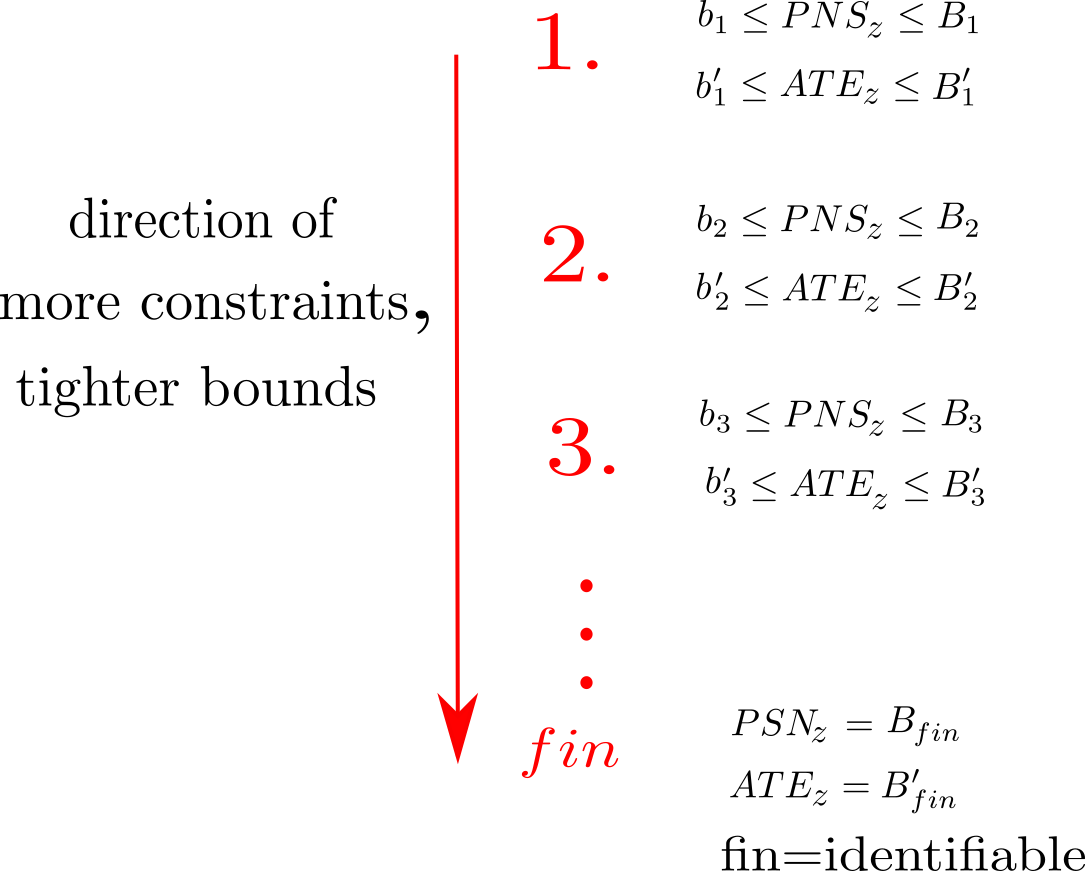
\includegraphics[width=3in]
{personalized/personalized-goal.png}
\caption{We use patient data
to calculate at each step, increasingly
tighter bounds
$b_j, b'_j, B_j, B'_j$
for $PNS_z$ and $ATE_z$,
ending in point bounds
for both quantities. }
\label{fig-personalized-goal}
\end{figure}

The goal of PTE theory, as
described by
Fig.\ref{fig-personalized-goal}, is
to find
increasingly
tighter bounds for
PTEs such as $PNS$,
$PNS_z$, $ATE$, $ATE_z$, etc..


We say bounds, because
it is not always possible
to give a point estimate
for $PNS$ and other
PTEs.
If a point estimate for a PTE named $Q$
is achievable, we say $Q$
is {\bf identifiable}.
The same definition
of identifiability
has been used before in this book
for $ATE$.
It's possible that
$ATE$ is identifiable,
but $PNS$ isn't,
or vice versa, for certain kinds
of data; i.e., both
quantities need not
become identifiable
simultaneous at the
same step above.


 The
bounds given by PTE theory
are
as tight as possible,
depending on
the available data,
and on what bnet model
assumptions
the user is willing to make.
We will consider two types of bounds:
(1) Bounds for an unspecified bnet,
(2) bounds for specific bnet families.
Bounds for (2) will be tighter
than bounds for (1).


The bounds are calculated from
 two types of data:
{\bf Observational Data (OD)} and
{\bf Experimental Data (ED)}.

For OD, one allows
the patient to
choose whether to take
a drug
or not ($x=0,1$),
and then we conduct a {\bf survey}
to record his/her
value for $x$
and whether the treatment
worked or not ($y=0,1$).

For ED, one conducts a {\bf RCT}
(Randomized Controlled Trial)
instead of a survey.
In the case of ED,
we record, as in OD, the $(x,y)$
for each patient, but
the value of $x$ for each
patient is selected by the
experimenter, at random,
and, once selected, it
 is compulsory for the
patient.

Unlike ED, OD is likely
to be confounded, but
it can still shed
additional information
that serves to tighten
the bounds on
$PNS_z$ or other PTEs.

OD is usually collected first
because it is easier and cheaper to collect
than ED. Sometimes ED is too expensive or difficult
or even impossible to collect,
so only OD is available.
Sometimes several ED (resp., several OD)
need to be merged, before merging
the merged ED with the merged OD. Pearl's PTE theory
allows us to fuse together all the
available data
in all these types of
situations.

Some purists such as the advocates of {\bf EBM (Evidence Based Medicine)}
advocate the use of only ED (i.e., only RCTs), no OD. This is reasonable in
certain administrative  professions to keep partisanship and chicanery out of
the decision making process, but in other professions, throwing away OD would
be foolish. Even in cases where an RCT is planned, a quick and cheap survey
can help design a better RCT. A case in the history of medicine where OD was
essential, was the case of John Snow (see Chapter \ref{ch-did}). John Snow
didn't have an RCT, but he was able to use OD to determine the driver of the
cholera epidemic in London. He saved countless lives by doing so. An EBM
purist would have thrown out his OD because it wasn't an RCT.

In the usual case, OD is collected first to aid in the design of an RCT, and
then an RCT is conducted to collect ED. In this case, an EBM purist would
throw away the OD, and only calculate an estimate of ATE.
What PTE theory
suggests is to calculate {\it both}, an estimate of ATE and bounds for PNS.
Why? Because ATE and PNS measure different things. ATE utilizes only ED
whereas PNS utilizes both OD and ED. Also, PNS is more personalized than ATE.

Some people object to PTE theory
and CI (Causal Inference) in general on the
grounds that the causal DAGs
 are adhoc, arbitrary, a
sort of unscientific voodoo. I think it’s because they fail to grasp the
following 3 things:

\begin{enumerate}

\item DAGs are not unique. Stop thinking that you have to find the unique
    DAG for the situation being considered. You just have to find a DAG
    that is a good causal fit for the situation. If a DAG is too
    complicated, you can always simplify it by merging several nodes into a
    single more abstract one, or by summing over unwanted nodes.

\item DAGs are roughly ordered from past to present. The arrows of a DAG
    roughly reflect the passage of time.

\item DAGs represent a scientific hypothesis that can and should be tested
    with do experiments.
\end{enumerate}



\section{Bnets for PTE theory}
\quad

Let $\ol{0}=1$ and $\ol{1}=0$.

Whenever we write $P(\rva=x, b)$,
we mean $P(\rva=x, \rvb=b)$.

In this chapter, we will
not use the notation
$P(y)$ and $P(y')$
used by Pearl to
discuss PTE theory.
Instead, we will
use $P(\rvy=1)$ and
$P(\rvy=0)$
to denote his
$P(y)$ and $P(y')$, respectively.


On the other hand,
in this chapter
we will change the names
of variables $\rvd, \rvy, \rvz, \rvy(d)$
used
in Chapter \ref{ch-pot-out} on Potential
Outcomes (PO)
to the names favored by Pearl.
Hence, we will replace
$\rvd, \rvy, \rvx, \rvy(d)$
by
$\rvx, \rvy, \rvz, \rvy_x$,
respectively.



PTE theory considers bnets of the form
Fig.\ref{fig-pte-bnet}.
The bnet considered in Rubin's
PO theory
is a very simple special case
of this where the box
labeled ``multiple nodes"
is absent and there is an
arrow pointing
from $\rvz$ to $\rvx$.


\begin{figure}[h!]
$$
\xymatrix{
&*++++[F]{\text{multiple nodes}}\ar@{<->}[ldd]
\ar@{<->}[r]
&*++[F-o]{\rvz}\ar[rd]\ar[d]
\\
&&\rvy_0\ar[d]
&\rvy_1\ar[ld]
\\
\rvx\ar[rr]
&&\rvy
}$$
\caption{Type of Bnet
considered in PTE theory.
The box labeled ``multiple nodes"
contains various observed
and hidden nodes with
arrows
to or from node $\rvx$
and to or from
node $\rvz$.
$\rvz$ can be a multinode.
$\rvz$
is shown
as hidden but
could be observed instead.
}
\label{fig-pte-bnet}
\end{figure}

The TPM, printed in blue,
 for node $\rvy$
of bnet Fig.\ref{fig-pte-bnet}
is as follows:


\beq\color{blue}
P(y|y_0, y_1, x)=\delta(y, y_x)
\label{eq-tpm-y-yx}
\eeq

This TPM is used
frequently
in PTE theory.  If $x,y_0, y_1$
are arguments
of $P()$, this TPM implies that one
can swap
$\rvy_x=y_x$
and $\rvy=y_x$
inside $P()$. For example,
\beqa
P(y_0,y_1,x)
&=&
P({\color{red}\rvy_x}=y_x,
 y_{\ol{x}},x)
\\
&=&
P({\color{red}\rvy}=y_x,
 y_{\ol{x}},x)
\eeqa

According to Pearl, the defining
property of $y_x$ is that


\beq
P(\rvy_x=y)=P(\rvy=y|\cald\rvx=x)
\label{eq-1st-law}
\eeq
Pearl likes to call
Eq.(\ref{eq-1st-law})
the 1st Law. The 1st Law is also a
consequence of bnet Fig.\ref{fig-pte-bnet}
and the TPM Eq.(\ref{eq-tpm-y-yx}).
Indeed,
$\cald\rvx=x$
means one should amputate
all arrows entering
node $\rvx$, and one should set
the TPM of $\rvx$ to a delta
function centered at $x$.
If that is done, then
the values
of $\rvy$ and $\rvy_x$ must
be equal,
because the TPM at node $\rvy$
is a delta function that
enforces this equality.

\section{$ATE = PNS - AMM$}

Define the {\bf Probability of Necessity and Sufficiency}
\beq
PNS = P(\rvy_0=0, \rvy_1=1)
\eeq
and the {\bf Amonotonicity Measure} by
\beq
AMM = P(\rvy_0=1, \rvy_1=0)
\eeq

\begin{claim}
\beq
PNS=P(\rvy_1-\rvy_0=1)
\eeq
\beq
AMM=P(\rvy_1-\rvy_0=-1)
\eeq
\end{claim}
\proof

$\rvy_1-\rvy_0=1$ iff ($\rvy_1=1$ and
$\rvy_0=0$).

$\rvy_1-\rvy_0=-1$ iff ($\rvy_1=0$ and
$\rvy_0=1$).
\qed

\begin{figure}[h!]
\centering
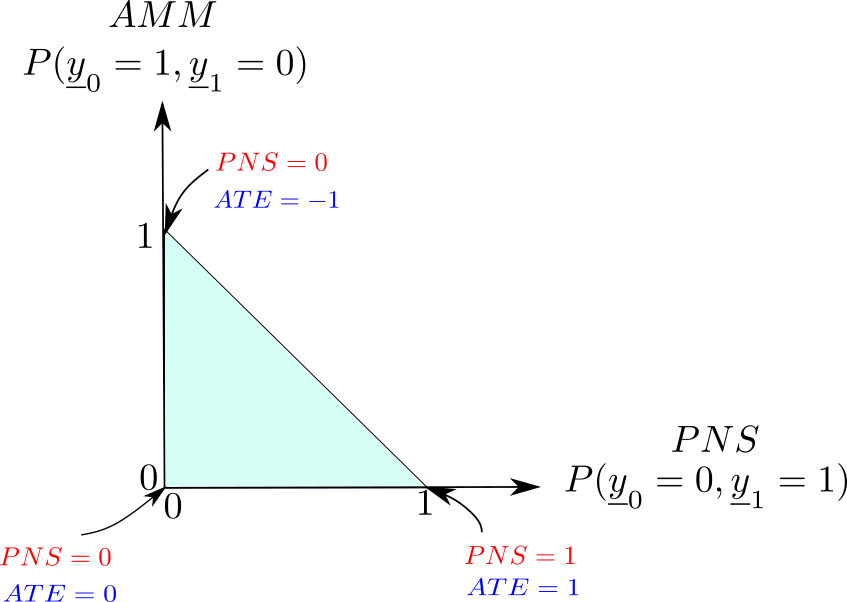
\includegraphics[width=3.5in]
{personalized/pns-ate.png}
\caption{Probability simplex
$\{(x,y): x\geq 0, y\geq 0, x+y\leq 1\}$
with $x=PNS$
and $y=AMM$.
Values of $PNS$ and $ATE$
at corners
are given.
Points on line $x+y=1$ can only be
achieved if $P(1,1)=P(0,0)=0$. }
\label{fig-pns-ate}
\end{figure}
\begin{claim}
\beq
ATE = PNS - AMM
\eeq
\end{claim}
\proof
\beqa
ATE &=& E_\s[y^\s_1-y^\s_0]
\\
&=&E[\rvy_1-\rvy_0]
\\
&=&
\sum_{y}y[P(\rvy_1=y) -P(\rvy_0=y)]
\\
&=&
P(\rvy_1=1) -P(\rvy_0=1)
\\
&=&
\sum_{y_0}P(y_0, \rvy_1=1) - \sum_{y_1}P(\rvy_0=1, y_1)
\\
&=&
\underbrace{P(\rvy_0=0, \rvy_1=1)}_{PNS} -
\underbrace{P(\rvy_0=1, \rvy_1=0)}_{AMM}
\eeqa
\qed



See Fig.\ref{fig-pns-ate}
for a visualization
of the extreme values of
$PNS$ and the corresponding values
of $ATE$.

\section{Probabilities Relevant to PTE theory}
Note\footnote{
To
translate this section
from
our notation
to the notation
used by Tian and Pearl in
Ref.\cite{pearl-tian-2000},
 replace $P(\rvy_1=i,
 \rvy_0=j, \rvx=k)\rarrow p_{i,j,k}$
$O_{1,0}\rarrow P(x,y') $,
$O_{0|1}\rarrow P(y'|x)$,
$ E_{0|1}\rarrow P(y'_x)$, etc.}

Let $x, y\in \bool$ and $z\in S_\rvz$ for
some finite, not necessarily binary set $S_\rvz$. Define
\beq
P^{x', y'}_{x,y}=
P(\rvy_{x'}=y'|x,y)
\eeq

{\bf observational (non-causal)
 probabilities}
\beq
O_{x,y}= P(\rvx=x,\rvy=y)
\eeq

\beq
O_{y|x}= P(\rvy=y|\rvx=x)
\eeq

\beq
\pi_x = P(\rvx=x)
\eeq

{\bf experimental (causal)
 probabilities}

\beq
E_{y|x}= P(\rvy_x=y)
\eeq

{\bf Average Treatment Effect (ATE)}
\beqa
ATE&=&
P(\rvy_1=1)-P(\rvy_0=1)
\\
&=&
E_{1|1}-E_{1|0}
\\
&=& E_{1|1}+E_{0|0}-1
\eeqa

{\bf Conditional ATE (CATE)}
\beqa
ATE_z&=&
P(\rvy_1=1|z)-P(\rvy_0=1|z)
\\
&=& E_{1|1,z}+E_{0|0,z}-1
\eeqa

{\bf Average Causal Effect}

\beq
ACE= P(\rvy=1|\cald\rvx=1)-P(\rvy=1|\cald\rvx=0)
\eeq
Note that
\beq
ACE=\underbrace{P(\rvy=1|\cald\rvx=1)}_{P(\rvy_1=1)}
-\underbrace{P(\rvy=1|\cald\rvx=0)}_{P(\rvy_0=1)}
=ATE\eeq

{\bf Conditional ACE
(CACE)}

This is what
is called
$ACE_z$ in Chapter \ref{ch-pot-out}.
Note that
$ACE_z=ATE_z$.

{\bf Effect of Treatment
 on the Treated (ETT)} (i.e., $ATE$
for  the treated)

\beq
ETT= \underbrace{P(\rvy_1=1|\rvx=1)}_
{\cale_1}
-\underbrace{P(\rvy_0=1|\rvx=1)}_{
\cale_0}
\eeq
Note that

\beqa
\cale_1\pi_1&=&
 P(\rvy_1=1, \rvx=1)
\\
&=&
O_{1,1}
\eeqa
and

\beqa
\cale_0\pi_1 &=&
P(\rvy_0=1,\rvx=1)
\\
&=& P(\rvy_0=1)-
\underbrace{P(\rvx=0, \rvy_0=1)}_{
P(\rvx=0, \rvy=1)}
\\&=&
E_{1|0}-O_{0,1}
\eeqa
so

\beq
ETT\pi_1= \sum_x O_{x, 1} -  E_{1|0}
\eeq



{\bf Probability of Necessity
($\PN$)}\footnote{I like to call
$PN$ the Probability of Nullifying, because
it goes from 11 to 00}
\beq
\PN = P^{0,0}_{1,1}
\eeq


{\bf Probability of Sufficiency
 ($\PS$)}\footnote{I like to call
$PS$ the Probability of Surging, because
it goes from 00 to 11}
\beq
\PS=P^{1,1}_{0,0}
\eeq




{\bf Probability of
Necessity and Sufficiency (PNS)}

\beq
PNS=
P(\rvy_0=0, \rvy_1=1)
\eeq

Henceforth, we will use $PNS3$ to
denote the trio

\beq
PNS3=(PNS, PN, PS)
\;.
\eeq

{\bf Amonotonicity Measure (AMM)}

\beq
AMM=
P(\rvy_0=1, \rvy_1=0)
\eeq

{\bf Risk ratio or relative risk (RR)}
\beq
RR = \frac{O_{1|1}}
{O_{1|0}}
\eeq



{\bf Excess Risk Ratio (ERR)}
\beq
ERR=
\frac{O_{1|1}-O_{1|0}}
{O_{1|1}}= 1 - \frac{1}{RR}
\eeq

{\bf Corrected ERR (CERR)}
\beq
CERR=
ERR +
\frac{O_{1|0}-E_{1|0}}{O_{1,1}}
\eeq

You might be wondering
how $P(\rvy_x=y|\rvx=0)$
and $P(\rvy_x=y|\rvx=1)$ for $x,y\in\bool^2$
are related to $O_{y|x}$ and $E_{y|x}$.
The following claim shows how.

\begin{claim}
\begin{subequations}
\label{eq-judeasrx-eqs}

\beq
P(\rvy_x=y|\rvx=x)=O_{y|x}
\eeq

\beq
P(\rvy_x=y|\rvx=\ol{x})=
\frac{E_{y|x}-O_{y|x}\pi_x}{\pi_{\ol{x}}}
\eeq
\end{subequations}
\end{claim}
\proof
Before we begin the proof, note
that summing both sides
of Eqs.(\ref{eq-judeasrx-eqs})
gives $1=1$, so these 2 equations
pass that test.

\beq
P(\rvy_x=y|\rvx=x)=P(\rvy=y|\rvx=x)=O_{y|x}
\eeq

\beqa
P(\rvy_x=y|\rvx=\ol{x})&=&
\frac{P(\rvy_x=y,\rvx=\ol{x})}
{\pi_{\ol{x}}}
\\
&=&
\frac{P(\rvy_x=y)-P(\rvy_x=y,\rvx=x)}
{\pi_{\ol{x}}}
\\
&=&
\frac{P(\rvy_x=y)-P(\rvy_x=y|\rvx=x)\pi_x}
{\pi_{\ol{x}}}
\\
&=&
\frac{E_{y|x}-O_{y|x}\pi_x}{\pi_{\ol{x}}}
\eeqa

\qed



\begin{claim}\label{cl-p-y0-y1-x}


\beqa
P(y_0, y_1|x)
&=&
P(y_{\ol{x}}|x, \rvy=y_x)P(\rvy=y_x|x)
\\
&&\xymatrix{\\=}
\xymatrix{
&y_{\ol{x}}
\\
x\ar[ur]\ar[r]
&\rvy=y_x\ar[u]
}
\eeqa
\end{claim}
\proof

\beqa
P(y_0, y_1|x)
&=&
\frac{P(y_0, y_1, x)}{P(x)}
\\
&=&
\frac{P(y_{\ol{x}}, x, \rvy=y_x)}{P(x)}
\\
&=&
\frac{P(y_{\ol{x}}|x, \rvy=y_x)P(x, \rvy=y_x)}{P(x)}
\\
&=&
P(y_{\ol{x}}|x, \rvy=y_x)P(\rvy=y_x|x)
\eeqa
\qed

\begin{claim}
\label{cl-y0-y1-separation}

\beq
\underbrace{PNS}_{
P(\rvy_0=0, \rvy_1=1)
}
=\PN *O_{1,1} +
\PS *O_{0,0}
\eeq
Hence, if we know
any two of $(\PN, \PS, PNS)$,
we can calculate the
third.
\end{claim}
\proof
\begin{align}
P(y_0,y_1)
&=
\sum_xP(y_0,y_1|x)P(x)
\\
&=
\sum_x P(y_{\ol{x}}|x, \rvy=y_x)P(x,\rvy=y_x)\quad
\text{(see Claim \ref{cl-p-y0-y1-x}.)}
\\&=
\left\{
\begin{array}{c}
\quad P(y_1|\rvx=0, \rvy=y_0)P(\rvx=0, \rvy=y_0)
\\
+ P(y_0|\rvx=1, \rvy=y_1)P(\rvx=1, \rvy=y_1)
\end{array}
\right.
\end{align}
Thus,

\begin{align}
P(\rvy_0=0, \rvy_1=1)
&=
\left\{
\begin{array}{c}
\quad P(\rvy_1=1|\rvx=0, \rvy=0)P(\rvx=0, \rvy=0)
\\
+ P(\rvy_0=0|\rvx=1, \rvy=1)P(\rvx=1, \rvy=1)
\end{array}
\right.
\\
&=
\PS *O_{0,0}
+
\PN *O_{1,1}
\end{align}
\qed

Note that $PNS$ refers to
both $\rvy_0$ and $\rvy_1$,
$\PN$ refers only to
$\rvy_0$ and $\PS$ refers only to
$\rvy_1$. Thus, $\PN$ and $\PS$
serve to separate the pair
of variables
$(\rvy_0, \rvy_1)$
and to isolate them individually.
Claim \ref{cl-y0-y1-separation}
is a quantitative expression of that
separation.

Pearl likes to say that
$PNS$ belongs to Rung 3 because it's a
probability that involves both
$\rvy_0$ and $\rvy_1$, and
one of those two must be a counterfactual
(an event that never occurred). On the
other hand, $\PN, \PS, ATE$, etc.,
are defined in terms of probabilities
that involve either $\rvy_0$
or $\rvy_1$ but not both.
Probabilities that
involve only one of them,
 can be
expressed with the do operator,
so they belong to Rung 2.
Conditional probabilities
like $P(y|x)$ that
involve neither $\rvy_0$
nor $\rvy_1$  belong to Rung 1.\footnote{
Probabilities
such as $P(\rvy_0=1,\rvy=0,\rvx=1)=
P(\rvy_0=1, \rvy_1=0, \rvx=1)$
are considered Rung 3.}






\section{Symmetry}


Define $\sim$ to
be an operator that swaps zeros and ones
in $P(\rvy_0=y, \rvy_1=y', x)$.
Hence

\beq
[P(\rvy_0=y, \rvy_1=y', \rvx=x)]^\sim=
P(\rvy_1=\ol{y}, \rvy_0=\ol{y'}, \rvx=\ol{x})
\eeq

\beq
(P^{x',y'}_{x,y})^\sim= P^{\ol{x'}, \ol{y'}}_{\ol{x}, \ol{y}}
\eeq

\beq
(O_{x,y})^\sim = O_{\ol{x},\ol{y}}
\eeq

\beq
(O_{y|x})^\sim = O_{\ol{y}|\ol{x}}
\eeq


\beq
(\pi_x)^\sim =\pi_{\ol{x}}
\eeq

\beq
(E_{y|x})^\sim = E_{\ol{y}|\ol{x}}
\eeq

\beq
(\PN)^\sim=\PS,\quad (\PS)^\sim=\PN
\eeq

\beq
(PNS)^\sim= PNS
\eeq

\beq
(RR)^\sim=
\frac{O_{0|0}}{O_{0|1}}
\eeq

Recall

\beq
ERR=\frac{O_{1|1}-O_{1|0}}{O_{1|1}}=1-\frac{1}{RR}
\eeq
Therefore, define

\beq
(ERR)^\sim=
\frac{O_{0|0}-O_{0|1}}
{O_{0|0}}
=1 - \frac{1}{(RR)^\sim}
\eeq

Note that

\beqa
O_{1|1}-O_{1|0}&=&
O_{1|1}+O_{0|0}-1
\\&=&
O_{0|0}-O_{0|1}
\\&=&
(O_{1|1}-O_{1|0})^\sim
\eeqa


\section{Linear Programming Problem}

{\bf Probability Simplex}

\beq
\cals=\left\{P(y_0,y_1, x):
\begin{array}{c}
P(y_0,y_1, x)\geq 0
\\
y_0, y_1, x\in\bool
\\
\sum_{y_0=0}^1
\sum_{y_1=0}^1
\sum_{x=0}^1
P(y_0,y_1, x)
=1
\end{array}
\right\}\eeq

Note that $\cals$ has 7 degrees of freedom (dofs).


\begin{enumerate}
\item
{\bf observational (non-causal)
 constraints on $\cals$}
{\color{red}(3 constraints)}

\beq
O_{x, y}=P(x,y)=
\sum_{y'}
P(\rvy_x=y, \rvy_{\ol{x}}=y', x)
\quad\text{for $(x,y)\in\{(0,1),(1,0),(1,1)\}$}
\eeq

\item
{\bf experimental (causal) constraints
  on $\cals$}
{\color{red}(2 constraints)}\footnote{
$E_{0|x}$ follows from
$E_{0|x}=1-E_{1|x}$.}

\beq
E_{1|x}=P(\rvy_x=1)=\sum_{x'}
\sum_{y'}
P(\rvy_x=1, \rvy_{\ol{x}}=y', \rvx=x') \quad \text{for $x\in\bool$}
\eeq


\end{enumerate}

$\cals$ has 7 dofs but the
3 observational constraints
reduce the number of dofs to 4.
The 5 observational
and experimental constraints
 reduce the number of dofs
to 2.
$\cals$ is embedded in $\RR^8$
and then the 6 constraints (unit
probability, 2 observational
and 3 experimental)
reduce it
 to the interior
of a  6 or less sided figure
 in $\RR^2$.

Henceforth, we will
refer to the observational
 and experimental
constraints together
as the {\bf minimal
constraints}.

This is half of a
linear programming problem. Recall
that a {\bf linear programming problem}
can be stated as finding the column vector
$\xi$ that minimizes
 a cost $\calc=c^T\xi$ subject to $A\xi=b$ and $\xi\geq 0$.
Here we have no cost function
or minimization, but we have
$A\xi=b$ and
$\xi\geq 0$ where
$\xi =[P(y_0, y_1, x)]_{\forall y_0, y_1, x}$.
Also
$b= [1,
O_{0,1}, O_{1,0}, O_{1,1},
E_{1|0}, E_{1|1}]^T$, and
$A=$ a matrix of zeros and ones.

Note that
\beqa
PNS &=&
P(\rvy_0=0,\rvy_1=1)
\\
&=&
\sum_x P(\rvy_0=0,\rvy_1=1, x)
\eeqa

\beqa
\PN
&=&
 P(\rvy_0=0|\rvx=1,\rvy=1)
\\
&=&
\frac{P(\rvy_0=0, \rvy_1=1, \rvx=1)
}{O_{1,1}}
\eeqa

\beqa
\PS
&=&
 P(\rvy_1=1|\rvx=0,\rvy=0)
\\
&=&
\frac{P(\rvy_0=0, \rvy_1=1, \rvx=0)
}{O_{0,0}}
\eeqa



\section{Special constraints}
\begin{itemize}
\item
{\bf Exogeneity (a.k.a., no-confounding)}
holds for simplex $\cals$
if
$\rvy_x\perp \rvx$ for $x\in\bool$.
 Hence

\beq
\underbrace{P(\rvy_x=1)}_{E_{1|x}}
=P(\rvy_x=1|x)=
\underbrace{P(\rvy=1|x)}_{O_{1|x}}
\quad \text{for $x\in \bool$}
\eeq
Exogeneity gives {\color{red}2 constraints}.

Note that exogeneity
is the same thing as identifiability
of $P(\rvy_x=y)=P(\rvy=y|\cald\rvx=x)$.
But identifiability
(i.e., do-identifiability) is a more
general concept. One can speak
of the identifiability of $P(y_x|z)$
or of $P(y_0, y_1, a)$, etc.
In general,
any expression with
do operators is do-identifiable
if it can be expressed
as an expression without
do-operators.

\item
{\bf Strong Exogeneity} holds
for simplex $\cals$
if $(\rvy_0, \rvy_1)_{joint}
\perp \rvx$. Hence

\beq
P(y_0,y_1|x)=P(y_0, y_1)
\label{eq-strong-exogen}
\eeq
Strong exogeneity gives {\color{red} 3 constraints}.
Strong exogeneity implies
exogeneity
but not the converse.\footnote{In
this book, we use both
$(\rva, \rvb)_\&\perp \rvx$
and $(\rva, \rvb)_{joint}\perp \rvx$.
When we write $(\rva, \rvb)_\&\perp \rvx$,
we mean that
$\rva\perp \rvx$
and $\rvb\perp\rvx$,
or, equivalently,
$P(a|x)=P(a)$
and $P(b|x)=P(b)$.
When we write
$(\rva, \rvb)_{joint}\perp \rvx$
or simply $(\rva, \rvb)\perp \rvx$,
we mean $P(a,b|x)=P(a,b)$.
Summing
$P(a,b|x)=P(a,b)$
over $a$ gives
$P(b|x)=P(b)$,
and summing it
over $b$ gives
$P(a|x)=P(a)$.
Hence we see that
 $(\rva, \rvb)_{joint}\perp \rvx$
implies
$(\rva, \rvb)_\&\perp \rvx$
but not the converse.
If $\rva$ and $\rvb$ are independent at
fixed $\rvx$ so that
$P(a,b|x)=P(a|x)P(b|x)$ then
$(\rva, \rvb)_{joint}\perp \rvx$
iff
$(\rva, \rvb)_\&\perp \rvx$
}
\item
{\bf Monotonicity}\footnote{
This property is called monotonicity
 because
it's equivalent to the statement
that $y_0^\s\leq y_1^\s$ for
all individuals $\s$
in the population.
Indeed, $y_0^\s\leq y_1^\s$
includes the 3 cases $(y_0^\s, y_1^\s)=
(0,0), (1, 1), (0,1)$, but
excludes the only other
case, namely $(1,0)$.}
 holds for simplex $\cals$ if

\beq AMM=P(\rvy_0=1,
 \rvy_1=0)=0\eeq\;.
Equivalently,

\beq
\sum_x P(\rvy_0=1, \rvy_1=0, x)=0
\eeq
which is true iff

\beq
 P(\rvy_0=1, \rvy_1=0, x)=0\quad
\text{for $x\in\bool$}
\eeq
Monotonicity gives {\color{red} 2
constraints}.

Note that when $AMM=0$, $PNS=ATE$.
\end{itemize}



\begin{claim}
Monotonicity and exogeneity
together imply strong exogeneity.
\end{claim}
\proof

This proof is presented here
for completeness. Later
on, we will give a much
simpler proof of this result.
I advise the reader to skip this proof
on first reading
of this chapter.

Let $a\in \bool$.
\beqa
P(\rvy_a=\ol{a}, x)&=&
\sum_{a'}P(\rvy_a=\ol{a}, \rvy_{\ol{a}}=a', x)
\\
&=&P(\rvy_a=\ol{a}, \rvy_{\ol{a}}=\ol{a}, x)
\quad\text{(by monotonicity)}
\eeqa
Thus,

\beq
P(\rvy_a=\ol{a}|\rvx=a)=P(\rvy_a=\ol{a},
 \rvy_{\ol{a}}=\ol{a}|\rvx=a)
\label{eq-pm-with-cond}
\eeq
and
\beq
P(\rvy_a=\ol{a})=P(\rvy_a=\ol{a},
 \rvy_{\ol{a}}=\ol{a})
\label{eq-pm-without-cond}
\eeq
By exogeneity,
the left hand side of Eq.(\ref{eq-pm-with-cond})
and the left hand side of Eq.(\ref{eq-pm-without-cond})
are equal,
so the right hand sides
of those equations must be equal too.

\beq
P(\rvy_a=\ol{a},
 \rvy_{\ol{a}}=\ol{a}|\rvx=a)=
P(\rvy_a=\ol{a},
 \rvy_{\ol{a}}=\ol{a})
\eeq
This immediately implies\footnote{
If $x\in \bool$
and $P(a|\rvx=0)=P(a)$,
then $P(a)- P(a,\rvx=0)=
P(a)[1-P(\rvx=0)]$,
so $ P(a,\rvx=1)= P(a)P(\rvx=1)$.
Hence, $P(a|\rvx=1)=P(a)$.}

\beq
P(\rvy_a=\ol{a},
 \rvy_{\ol{a}}=\ol{a}|x)=
P(\rvy_a=\ol{a},
 \rvy_{\ol{a}}=\ol{a})
\eeq
for $x\in \bool$.
This gives for $a=0$
\beq
P(\rvy_0=1,
 \rvy_{1}=1|x)=
P(\rvy_0=1,
 \rvy_{1}=1)
\eeq
and for $a=1$
\beq
\underbrace{P(\rvy_1=0,
 \rvy_{0}=0|x)}_{
P(
 \rvy_{0}=0, \rvy_1=0|x)
}
=
\underbrace{
P(\rvy_1=0,
 \rvy_{0}=0)}_{P(\rvy_{0}=0,\rvy_1=0)}
\eeq
Monotonicity itself gives

\beq
 P(\rvy_0=1, \rvy_1=0|x)=0=
P(\rvy_0=1, \rvy_1=0)
\eeq
The remaining strong exogeneity constraint, given by
\beq
 P(\rvy_0=0, \rvy_1=1|x)=P(\rvy_0=0, \rvy_1=1)
\;,
\eeq
follows because
\beq
\sum_{y_0,y_1}P(y_0, y_1|x)=
\sum_{y_0,y_1}P(y_0, y_1)=1
\eeq

\qed


\section{Matrix representation of probabilities}

Suppose $\eps_x(y_0, y_1)$
for $x,y_0,y_1\in \bool$
 are eight vectors
in a vector space $V$.
$\eps_x(y_0, y_1)$ will only be used
at position $(y_0,y_1)$
of a $2\times 2$ matrix,
where the positions are
 defined as follows:

\beq
\xymatrix@R=.7pc@C=.7pc{
y_1
\\
1\ar[u]
&(0,1)
&(1,1)
\\
0\ar@{-}[u]
&(0,0)
&(1,0)
\\
\ar@{-}[u]
\ar@{-}[r]
&0\ar@{-}[r]
&1\ar[r]
&y_0
}
\eeq
When $\eps_x(y_0, y_1)$
is used inside a $2\times 2$
matrix, we will not write
the argument $(y_0, y_1)$,
leaving it implicit, unless
confusion may arise.
Thus, for example, we will
represent $\Pmat{\eps_0(0,1)}{0}{0}{0}$
by $\Pmat{\eps_0}{0}{0}{0}$.



For $x\in \bool$, let
\begin{subequations}
\beq
P_{\rvy_0, \rvy_1, \rvx}(0,0,x)=
\Pmat{0}{0}{\eps_x}{0}
\eeq

\beq
P_{\rvy_0, \rvy_1, \rvx}(0,1,x)=
\Pmat{\eps_x}{0}{0}{0}
\eeq

\beq
P_{\rvy_0, \rvy_1, \rvx}(1,0,x)=
\Pmat{0}{0}{0}{\eps_x}
\eeq


\beq
P_{\rvy_0, \rvy_1, \rvx}(1,1,x)=
\Pmat{0}{\eps_x}{0}{0}
\eeq
\label{eq-prob-mats}
\end{subequations}


Define a map
$\calp[\quad]:V\rarrow \RR$
that we will call the
{\bf matrix representation
of probabilities (MRP)} (mnemonic, Mr. P).
We will
assume that the map $\calp[\quad]$ is linear.
Hence, for instance,

\beq
\Pmat{4\eps_0+3\eps_1}
{-5\eps_0}
{0}
{0}=
4\Pmat{\eps_0}
{0}
{0}
{0}
+
3\Pmat{\eps_1}
{0}
{0}
{0}
-5
\Pmat{0}
{\eps_0}
{0}
{0}
\eeq

Henceforth, we will use the abbreviation

\beq
\eps_+ = \eps_0+\eps_1
\eeq

Note that

\beq
\Pmat{\eps_+}
{\eps_+}
{\eps_+}
{\eps_+}=1
\eeq

\beq
\pi_x=
\Pmat{\eps_x}
{\eps_x}
{\eps_x}
{\eps_x}
\eeq


\beq
E_{0|0}
=\Pmat{\eps_+}{0}{\eps_+}{0}
,\quad
O_{0,0}
=\Pmat{\eps_0}{0}{\eps_0}{0}
\eeq

\beq
E_{0|1}
=\Pmat{0}{0}{\eps_+}{\eps_+}
,\quad
O_{1,0}
=\Pmat{0}{0}{\eps_1}{\eps_1}
\eeq

\beq
E_{1|0}=\Pmat{0}{\eps_+}{0}{\eps_+}
,\quad
O_{0,1}=\Pmat{0}{\eps_0}{0}{\eps_0}
\eeq

\beq
E_{1|1}=\Pmat{\eps_+}{\eps_+}{0}{0}
,\quad
O_{1,1}=\Pmat{\eps_1}{\eps_1}{0}{0}
\eeq

\beq
P(\rvy=0)=O_{0,0}+O_{1,0}=
\Pmat{\eps_0}{0}{\eps_+}{\eps_1}
\eeq

\beq
P(\rvy=1)=O_{0,1}+O_{1,1}=
\Pmat{\eps_1}{\eps_+}{0}{\eps_0}
\eeq


\beq
\PN *O_{1,1}=\Pmat{\eps_0}{0}{0}{0}
\eeq

\beq
\PS *O_{0,0}=\Pmat{\eps_1}{0}{0}{0}
\eeq

\beq
PNS =\Pmat{\eps_+}{0}{0}{0}
\eeq

\beq
AMM =\Pmat{0}{0}{0}{\eps_+}
\eeq

\beq
ATE=PNS-AMM=
\Pmat{\eps_+}{0}{0}{-\eps_+}
\eeq


When $AMM=0$,
\beq
P(\rvy=1)|_{AMM=0}=
\Pmat{\eps_1}{\eps_+}{0}{0}
\eeq

The special constraints
of exogeneity, strong
exogeneity and
monotonicity have a very simple
in the
MRP.

Suppose that $\pi_0, \pi_1\geq 1$
and $\pi_0+\pi_1=1$. Note that
\beq
\left.
\begin{array}{c}
\eps_+ = \frac{\eps_0}{\pi_0}
\\
\text{or}
\\
\eps_+ = \frac{\eps_1}{\pi_1}
\end{array}
\right\}
\implies
\eps_+ = \frac{\eps_0}{\pi_0}
= \frac{\eps_1}{\pi_1}
\eeq

Below, we will abbreviate

\beq
\hat{\eps}_x =\frac{\eps_x}{\pi_x}
\eeq
for $x\in\bool$.


\begin{claim}
\label{cl-mrp-exo-mon}

\quad
\begin{enumerate}[(a)]
\item
Exogeneity holds iff (``4 sides can change
 color")

\begin{subequations}
\label{eq-mrp-exo}
\beq\Pmat{\hat{\eps}_0}{0}{\hat{\eps}_0}{0}=
 \Pmat{\hat{\eps}_1}{0}{\hat{\eps}_1}{0}
=
\Pmat{\eps_+}{0}{\eps_+}{0}
\eeq

\beq\Pmat{\hat{\eps}_0}{\hat{\eps}_0}{0}{0}=
 \Pmat{\hat{\eps}_1}{\hat{\eps}_1}{0}{0}
=
 \Pmat{\eps_+}{\eps_+}{0}{0}
\eeq

\beq\Pmat{0}{\hat{\eps}_0}{0}{\hat{\eps}_0}=
 \Pmat{0}{\hat{\eps}_1}{0}{\hat{\eps}_1}
=
\Pmat{0}{\eps_+}{0}{\eps_+}
\eeq

\beq\Pmat{0}{0}{\hat{\eps}_0}{\hat{\eps}_0}=
 \Pmat{0}{0}{\hat{\eps}_1}{\hat{\eps}_1}
\Pmat{0}{0}{\eps_+}{\eps_+}
\eeq
\end{subequations}

\item Monotonicity holds iff
\beq\Pmat{0}{0}{0}{\eps_x}=0
\eeq
for $x\in \bool$.

\item Strong exogeneity holds
 iff (``4 corners can change color")

\begin{subequations}
\label{eq-mrp-strong-exo}
\beq\Pmat{\hat{\eps}_0}{0}{0}{0}=
 \Pmat{\hat{\eps}_1}{0}{0}{0}=
\Pmat{\eps_+}{0}{0}{0}
\eeq

\beq\Pmat{0}{\hat{\eps}_0}{0}{0}=
 \Pmat{0}{\hat{\eps}_1}{0}{0}=
\Pmat{0}{\eps_+}{0}{0}
\eeq

\beq\Pmat{0}{0}{0}{\hat{\eps}_0}=
 \Pmat{0}{0}{0}{\hat{\eps}_1}=
 \Pmat{0}{0}{0}{\eps_+}
\eeq

\beq\Pmat{0}{0}{\hat{\eps}_0}{0}=
 \Pmat{0}{0}{\hat{\eps}_1}{0}=
\Pmat{0}{0}{\eps_+}{0}
\eeq
\end{subequations}


\end{enumerate}

\end{claim}
\proof

(a) This follows from
the definitions
of $E_{y|x}$ and $O_{x,y}$
for $x,y\in \bool$,
as stated above
in the MRP.

(b) This follows from the
identity
\beq
P_{\rvy_0, \rvy_1, \rvx}(1,0|x)=
\Pmat{0}{0}{0}{\frac{\eps_x}{\pi_x}}
\eeq
for $x\in\bool$.

(c) This follows from
definitions of $P_{\rvy_0, \rvy_1, \rvx}
(y_0, y_1, x)$ for $y_0, y_1, x\in \bool$,
as stated above
in the MRP.
\qed

Note that it is obvious
from Claim \ref{cl-mrp-exo-mon}
that strong exogeneity
implies exogeneity.

 Claim \ref{cl-mrp-exo-mon}
also makes it easy peasy
to prove that
exogeneity and monotonicity
imply strong exogeneity. Indeed,
here is a much simpler
proof than the one
we presented earlier.
\begin{claim}
Exogeneity and monotonicity
imply strong exogeneity.
\end{claim}
\proof
Let's call $E(a), E(b),
E(c), E(d)$ the four Eqs.(\ref{eq-mrp-exo})
that define Exogeneity,
and
$SE(a), SE(b),
SE(c), SE(d)$ the four
Eqs.(\ref{eq-mrp-strong-exo})
that define Strong Exogeneity.
\begin{itemize}
\item
Monotonicity implies the lower right
entry is zero, so $SE(c)$ is true.

\item
Setting to zero
the lower right entry in $E(c)$ and $E(d)$
 implies $SE(b)$ and $SE(d)$.

\item Subtracting $SE(d)$ from $E(a)$
gives $SE(a)$.
\end{itemize}
\qed

\section{Bounds on Exp. Probs. imposed by Obs. Probs.}

\begin{claim}
In general,

\beq
O_{x,1}\leq E_{1|x} \leq 1-O_{x,0}
\quad\text{for $x\in \bool$}
\;.
\eeq
In other words,

\beq
O_{1,1}\leq E_{1|1} \leq 1-O_{1,0}
\eeq
\beq
O_{0,1}\leq E_{1|0} \leq 1-O_{0,0}
\eeq
With monotonicity, we get the tighter bounds

\beq
\overbrace{
O_{1,1} +
\underbrace{O_{0,1}}_{new}
}^{P(\rvy=1)}
\leq
E_{1|1}\leq 1- O_{1,0}
\eeq
\beq
O_{0,1}\leq E_{1|0}
\leq
\overbrace{
1- O_{0,0}-\underbrace{O_{1,0}}_{new}
}^{P(\rvy=1)}
\eeq

\end{claim}
\proof

\beq
O_{1,1}\leq E_{1|1} \leq
\underbrace{1-O_{1,0}}
_{O_{1,1}+O_{0,0}+O_{0,1}}
\eeq
has the MRP


\beq
\Pmat{\eps_1}{\eps_1}{0}{0}
\leq
\Pmat{\eps_+}{\eps_+}{0}{0}
\leq
\Pmat{\eps_1}{\eps_1}{0}{0}
+
\Pmat{\eps_0}{0}{\eps_0}{0}
+
\Pmat{0}{\eps_0}{0}{\eps_0}
\eeq
which is obviously true.

\beq
O_{0,1}\leq E_{1|0} \leq
\underbrace{1-O_{0,0}}
_{O_{1,1}+O_{0,1}+O_{1,0}}
\eeq
has the MRP

\beq
\Pmat{0}{\eps_0}{0}{\eps_0}
\leq
\Pmat{0}{\eps_+}{0}{\eps_+}
\leq
\Pmat{\eps_1}{\eps_1}{0}{0}
+
\Pmat{0}{\eps_0}{0}{\eps_0}
+
\Pmat{0}{0}{\eps_1}{\eps_1}
\eeq
which is obviously true.

\beq
P(\rvy=1)|_{AMM=0}\leq E_{1|1}
\eeq
has the MRP

\beq
\Pmat{\eps_1}{\eps_+}{0}{0}
\leq
\Pmat{\eps_+}{\eps_+}{0}{0}
\eeq
which is obviously true.

\beq
E_{1|0}|_{AMM=0}\leq
P(\rvy=1)|_{AMM=0}
\eeq
has the MRP

\beq
\Pmat{0}{\eps_+}{0}{0}
\leq
\Pmat{\eps_1}{\eps_+}{0}{0}
\eeq
which is obviously true.
\qed



\section{Bounds on $PNS3$ for unspecified bnet}

\begin{claim}\label{cl-basic-bound-joint}
If $P(a,b)$ is a probability
distribution, then
\beq
\max\{0, P(a) + P(b)-1\}\leq
P(a,b)\leq \min\{P(a), P(b)\}
\eeq
\end{claim}
\proof
$P(a|b)\leq 1$
and $P(b|a)\leq 1$
implies $P(a,b)\leq P(b)$
and $P(a,b)\leq P(a)$.
Hence, $P(a,b)\leq \min\{P(a), P(b)\}$.

\begin{align}
P(a) + P(b) -1
&=
\sum_{a', b'} P(a',b')
\underbrace
{[\delta(a,a')+\delta(b,b')
-1]}_{T}
\\
&\leq
P(a,b)\quad
\text{($T$ biggest
when $a=a'$ and $b=b'$)}
\end{align}
\qed


\begin{figure}[h!]
\centering
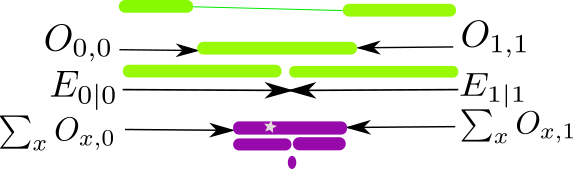
\includegraphics[width=3in]
{personalized/bounds-minimal.png}
\caption{Minimal bounds
for $PNS$.
$PNS$ is larger
than maximum of the purple segments
and smaller than the
minimum of the green ones.
The purple segment of almost zero
length represents zero.
The green segment
interrupted by a thin green
line represents $O_{0,0} + O_{1,1}$.
Note that $\sum_x O_{x,0}+
\sum_x O_{x,1}=1$. When
monotonicity holds,
$PNS$ equals $E_{1,1}+E_{0,0}-1$
which is the purple
segment marked with a star.
}
\label{fig-bounds-minimal}
\end{figure}

\begin{claim} Minimal bounds
\label{cl-minimal-bounds}
(see Fig.\ref{fig-bounds-minimal})

If the minimal
constraints hold for simplex $\cals$,
then

\beq
\max\left\{
\begin{array}{c}
0
\\
E_{1|1}+E_{0|0}-1
\\
E_{0|0}-\sum_x O_{x,0}
\\
E_{1|1}-\sum_x O_{x,1}
\end{array}
\right\}
\leq
PNS
\leq
\min\left\{
\begin{array}{c}
E_{1|1}
\\
E_{0|0}
\\
O_{1,1}+O_{0,0}
\\
E_{1|1}+E_{0|0}-O_{1,1}-O_{0,0}
\end{array}
\right\}
\eeq

\beq
\max\left\{
\begin{array}{c}
0
\\
\frac{E_{0|0}-\sum_x O_{x,0}}
{O_{1,1}}
\end{array}
\right\}
\leq
\PN
\leq
\min\left\{
\begin{array}{c}
1
\\
\frac{E_{0|0}-O_{0,0}}
{O_{1,1}}
\end{array}
\right\}
\eeq

\beq
\max\left\{
\begin{array}{c}
0
\\
\frac{E_{1|1}-\sum_x O_{x,1}}
{O_{0,0}}
\end{array}
\right\}
\leq
\PS
\leq
\min\left\{
\begin{array}{c}
1
\\
\frac{E_{1|1}-O_{1,1}}
{O_{0,0}}
\end{array}
\right\}
\eeq
\end{claim}
\proof
These bounds
were copied directly
from Ref.\cite{pearl-tian-2000},
except the notation was changed.
In certain cases, we have slightly
rewritten
the bounds
from Ref.\cite{pearl-tian-2000} to
 exhibit more explicitly their
symmetry under swaps of zeros and ones.
For example,
instead of using
$(E_{1|0}, E_{1|1})$
as parameters,
we use $(E_{1|1}, E_{0|0})$.

These bounds are obviously true
in the MRP. Indeed, in the MRP,
the following holds. For $PNS$, we have

\beq
\left[
\begin{array}{c}
0
\\
\\
E_{1|1}+ E_{0|0}-1
\\
\\
E_{0|0} -\sum_x O_{x,0}
\\
\\
E_{1|1} -\sum_x O_{x,1}
\end{array}
\right]
=
\left[
\begin{array}{c}
0
\\
\Pmat{\eps_+}{0}{0}{-\eps_+}
\\
\Pmat{\eps_1}{0}{0}{-\eps_1}
\\
\Pmat{\eps_0}{0}{0}{-\eps_0}
\end{array}
\right]
\eeq

\beq
PNS =
\Pmat{\eps_+}{0}{0}{0}
\eeq

\beq
\left[
\begin{array}{c}
E_{1|1}
\\
\\
E_{0|0}
\\
\\
O_{1,1}+ O_{0,0}
\\
\\
E_{1|1} + E_{0|0}
-O_{1,1}- O_{0,0}
\end{array}
\right]
=
\left[
\begin{array}{c}
\Pmat{\eps_+}{0}{\eps_+}{0}
\\
\Pmat{\eps_+}{\eps_+}{0}{0}
\\
\Pmat{\eps_+}{\eps_1}{\eps_0}{0}
\\
\Pmat{\eps_+}{\eps_0}{\eps_1}{0}
\end{array}
\right]
\eeq

For $\PN$, we have

\beq
\left[
\begin{array}{c}
0
\\
\\
E_{1|1} -\sum_x O_{x,1}
\end{array}
\right]
=
\left[
\begin{array}{c}
0
\\
\Pmat{\eps_0}{0}{0}{-\eps_0}
\end{array}
\right]
\eeq


\beq
\PN *O_{1,1}=\Pmat{\eps_0}{0}{0}{0}
\eeq

\beq
\left[
\begin{array}{c}
1
\\
\\
E_{1|1} - O_{1,1}
\end{array}
\right]
=
\left[
\begin{array}{c}
1
\\
\Pmat{\eps_0}{\eps_0}{0}{0}
\end{array}
\right]
\eeq


For $\PS$, we have

\beq
\left[
\begin{array}{c}
0
\\
\\
E_{0|0} -\sum_x O_{x,0}
\end{array}
\right]
=
\left[
\begin{array}{c}
0
\\
\Pmat{\eps_1}{0}{0}{-\eps_1}
\end{array}
\right]
\eeq


\beq
\PS *O_{0,0}=\Pmat{\eps_1}{0}{0}{0}
\eeq

\beq
\left[
\begin{array}{c}
1
\\
\\
E_{0|0} - O_{0,0}
\end{array}
\right]
=
\left[
\begin{array}{c}
1
\\
\Pmat{\eps_1}{\eps_1}{0}{0}
\end{array}
\right]
\eeq


The first two lines of the
bound for $PNS$ are a simple
consequence of
Claim \ref{cl-basic-bound-joint}.
Indeed, Claim \ref{cl-basic-bound-joint}
implies
\beq
\max\left\{\begin{array}{c}
0\\
 P(y_0)+P(y_1)-1
\end{array}\right\}
\leq
P(y_0, y_1)
\leq
\min\left\{\begin{array}{c}
P(y_0)\\
 P(y_1)
\end{array}\right\}
\eeq
When $y_0=0, y_1=1$, we get
\beq
\max\left\{\begin{array}{c}
0\\
 E_{0|0}+E_{1|1}-1
\end{array}\right\}
\leq
PNS
\leq
\min\left\{\begin{array}{c}
 E_{0|0}\\
 E_{1|1}
\end{array}\right\}
\eeq
\qed


In  Claim \ref{cl-minimal-bounds},
note that


\begin{itemize}
\item $\sum_x O_{x,y}=P(\rvy=y)$
for $y=0,1$.

\item Let

\beq
E'_{0|0}=E_{0|0}-\sum_x O_{x,0}
=\Pmat{\eps_1}{0}{0}{-\eps_1}
\eeq

\beq
E'_{1|1}=E_{1|1}-\sum_x O_{x,1}
=\Pmat{\eps_0}{0}{0}{-\eps_0}
\eeq


\beq
ATE=E_{1|1}+E_{0|0}-1=E'_{1|1}+E'_{0|0}=
\Pmat{\eps_+}{0}{0}
{-\eps_+}
\eeq

\item Claim \ref{cl-minimal-bounds}
applies if we have both observational
data (OD)
and experimental data (ED). If we only have
OD (resp., ED), ignore all
bounds that involve an $E$
(resp., involve an $O$) probability.

Hence, with only OD\footnote{The
bounds Eq.(\ref{eq-nds-only-od})
assume exogeneity does not hold.
For the case
when exogeneity does hold,
stronger bounds
will be given later on in the chapter.}

\beq
0\leq PNS \leq O_{1,1} + O_{0,0}
\label{eq-nds-only-od}
\eeq

and
$\PN,\PS\in[0,1]$,
whereas with only ED,
\beq
\max\left\{
\begin{array}{c}
0
\\
E_{1|1}+E_{0|0}-1
\end{array}
\right\}
\leq
PNS
\leq
\min\left\{
\begin{array}{c}
E_{1|1}
\\
E_{0|0}
\end{array}
\right\}
\eeq
and
$\PN,\PS\in[0,1]$.

\item At first blush, there seem to be
 3 possible cases to
consider: (1) Only OD. (2) Both OD and ED.
(3) Only ED.
Actually, Case (1) plus the assumption of
 exogeneity is the same as Case (3). Indeed,
recall that exogeneity means
no confounding, and ED (i.e., an RCT) also
has no confounding. So we don't have to consider
Case (3) if we consider Case (1) without and with
exogeneity. Exogeneity
is built into case (2), so case (2)
without exogeneity is meaningless.

\end{itemize}




\begin{claim}\label{cl-personal-exogen}
If minimal
and exogeneity constraints hold
for simplex $\cals$, then


\beq
\max\left\{
\begin{array}{c}
0
\\
O_{1|1}+O_{0|0}-1
\\
\cancel{O_{0|0}-\sum_x O_{x,0}}
\\
\cancel{O_{1|1}-\sum_x O_{x,1}}
\end{array}
\right\}
\leq
PNS
\leq
\min\left\{
\begin{array}{c}
O_{1|1}
\\
O_{0|0}
\\
\cancel{O_{1,1}+O_{0,0}}
\\
\cancel{O_{1|1}+O_{0|0}-O_{1,1}-O_{0,0}}
\end{array}
\right\}
\eeq


\beq
\max\left\{\begin{array}{c}
0\\
ERR
\end{array}\right\}
\leq
\PN
\leq
\min\left\{\begin{array}{c}
1\\
\frac{O_{0|0}}{O_{1|1}}
\end{array}\right\}
\eeq

\beq
\max\left\{\begin{array}{c}
0\\
(ERR)^\sim
\end{array}\right\}
\leq
\PS
\leq
\min\left\{\begin{array}{c}
1\\
\frac{O_{1|1}}{O_{0|0}}
\end{array}\right\}
\eeq

\end{claim}
\proof
Just
replace $E_{y|x}$ by $O_{y|x}$
in the minimal bounds given in
Claim \ref{cl-minimal-bounds}.

The canceled terms do not
improve the bounds and can be dropped.
We show this next using MRP.

In the MRP, the minimal bounds
for $PNS$ are
\beq
\left[
\begin{array}{c}
0
\\
\\
E_{1|1}+ E_{0|0}-1
\\
\\
E_{0|0} -\sum_x O_{x,0}
\\
\\
E_{1|1} -\sum_x O_{x,1}
\end{array}
\right]
=
\left[
\begin{array}{c}
0
\\
\Pmat{\eps_+}{0}{0}{-\eps_+}
\\
\Pmat{\eps_1}{0}{0}{-\eps_1}
\\
\Pmat{\eps_0}{0}{0}{-\eps_0}
\end{array}
\right]
\eeq

\beq
PNS =
\Pmat{\eps_+}{0}{0}{0}
\eeq

\beq
\left[
\begin{array}{c}
E_{1|1}
\\
\\
E_{0|0}
\\
\\
O_{1,1}+ O_{0,0}
\\
\\
E_{1|1} + E_{0|0}
-O_{1,1}- O_{0,0}
\end{array}
\right]
=
\left[
\begin{array}{c}
\Pmat{\eps_+}{0}{\eps_+}{0}
\\
\Pmat{\eps_+}{\eps_+}{0}{0}
\\
\Pmat{\eps_+}{\eps_1}{\eps_0}{0}
\\
\Pmat{\eps_+}{\eps_0}{\eps_1}{0}
\end{array}
\right]
\eeq
If exogeneity holds,
we can replace all $E$'s
by $O$'s on the left hand sides.
We can also use $\eps_+=\hat{\eps}_0=
\hat{\eps}_1$
on the right hand sides to conclude that

\beq
O_{1|1}+O_{0|0}-1=
\Pmat{\eps_+}
{\eps_+-\eps_+}
{0}
{-\eps_+}
=
\Pmat{\hat{\eps}_x}
{\hat{\eps}_x-\hat{\eps}_x}
{0}
{-\hat{\eps}_x}
=
\frac{1}{\pi_x}
\Pmat{\eps_x}
{0}
{0}
{-\eps_x}
\eeq
for both $x\in\bool$.
Note that
$\frac{1}{\pi_x}\Pmat{\eps_x}{0}{0}{-\eps_x}$
will always be greater or equal to
$\Pmat{\eps_x}{0}{0}{-\eps_x}$
when $\Pmat{\eps_x}{0}{0}{-\eps_x}\geq 0$ (if it's
negative, the 0 bound takes precedence). Hence,
the two canceled lower bound terms
can be dropped.
A similar argument shows that the
two canceled upper bound terms
can be dropped too.
\qed



\begin{claim}
If the minimal and
strong exogeneity constraints
 hold for simplex $\cals$,
then the inequalities
for exogeneity Claim \ref{cl-personal-exogen}
hold.
In addition,
\beq
\PN =\frac{PNS}{O_{1|1}}
\eeq
and

\beq
\PS =\frac{PNS}{O_{0|0}}
\eeq
\end{claim}
\proof
\beqa
\PN *O_{1|1}&=&
P(\rvy_0=0, \rvy=1|\rvx=1)
\\
&=&
P(\rvy_0=0, \rvy_1=1)
\\
&=&PNS
\eeqa

\beqa
\PS *O_{0|0}&=&
P(\rvy_1=1, \rvy=0|\rvx=0)
\\
&=&
P(\rvy_0=0, \rvy_1=1)
\\
&=& PNS
\eeqa
\qed


\begin{claim}\label{cl-pm-mono}
If the minimal
and monotonicity constraints hold
 for simplex $\cals$, then




\beq
PNS=E_{1|1}+E_{0|0}-1
\eeq

\beq
\PN =\frac{E_{0|0}-\sum_x O_{x,0}}{O_{1,1}}
=
\frac{\sum_x O_{x,1}-E_{1|0}}{O_{1,1}}
=
CERR
\eeq

\beq
\PS = \frac{E_{1|1}-\sum_x O_{x,1}}{O_{0,0}}
= \frac{\sum_x O_{x,0}-E_{0|1}}{O_{0,0}}
= (CERR)^\sim
\eeq



\end{claim}
\proof
These results can be easily
proven using the MRP.

Note that

\beqa
\frac{\sum_x O_{x,1}-E_{1|0}}{O_{1,1}}
&=&
\frac{ O_{1|1}\pi_1 + O_{1|0}(1-\pi_1)
-E_{1|0}}{O_{1|1}\pi_1}
\\
&=&
1-\frac{O_{1|0}}{O_{1|1}}
+\frac{O_{1|0}-E_{1|0}}{O_{1,1}}
\\
&=& CERR
\eeqa

\qed


\begin{claim}
If the minimal,
exogeneity and monotonicity
constraints hold
 for simplex $\cals$, then
$PNS$, $\PN$,$\PS$ are identifiable,
and


\beq
PNS = O_{1|1}+O_{0|0}-1
\eeq

\beq
\PN
=\frac{O_{0|0}-\sum_x O_{x, 0}}{O_{1,1}}
=\frac{\sum_x O_{x, 1}-O_{1|0}}{O_{1,1}}
=ERR
\eeq

\beq
\PS=\frac{O_{1|1}-\sum_x O_{x,1}}{O_{0,0}}
=\frac{\sum_x O_{x,0}-O_{0|1}}{O_{0,0}}
=(ERR)^\sim
\eeq

\end{claim}
\proof
Set $E_{y|x}=O_{y|x}$ in Claim
\ref{cl-pm-mono}.
\qed

\section{Bounds on $PNS3$
for specific bnet families}
Define
\beq
E_{*|*,z} = E_{0|0, z} + E_{1|1, z}=ATE_z+1
\eeq

\beq
O_{*,*|z} = O_{0,0|z} + O_{1,1| z}
\eeq


\begin{claim}\label{cl-pre-backdoor-bounds}
If $\rvz\cap de(\rvx)=\emptyset$, then
\beq
\max\left\{
\begin{array}{c}
0\\
E_{*|*,z}-1
\\
E_{0|0,z}-\sum_x O_{x,0|z}
\\
E_{1|1,z}-\sum_x O_{x,1|z}
\end{array}
\right\}
\leq
PNS_z
\leq
\min\left\{
\begin{array}{c}
E_{1|1,z}
\\
E_{0|0,z}
\\
O_{*,*|z}
\\
E_{*|*,z}-O_{*,*|z}
\end{array}
\right\}
\label{eq-pre-backdoor-bounds}
\eeq

\beq
\max\left\{
\begin{array}{c}
0
\\
\frac{E_{0|0,z}-\sum_x O_{x,0|z}}
{O_{1,1|z}}
\end{array}
\right\}
\leq
PN_z
\leq
\min\left\{
\begin{array}{c}
1
\\
\frac{E_{0|0, z}-O_{0,0|z}}
{O_{1,1|z}}
\end{array}
\right\}
\eeq

\beq
\max\left\{
\begin{array}{c}
0
\\
\frac{E_{1|1,z}-\sum_x O_{x,1|z}}
{O_{0,0|z}}
\end{array}
\right\}
\leq
PS_z
\leq
\min\left\{
\begin{array}{c}
1
\\
\frac{E_{1|1,z}-O_{1,1|z}}
{O_{0,0|z}}
\end{array}
\right\}
\eeq
\end{claim}
\proof
These are just the minimal bounds
where everything is conditioned on $z$.
\qed

In the minimal bounds, node $\rvz$
is not mentioned because
the minimal bounds don't assume
that $\rvz$ exists.
Once we assume that
node $\rvz$ exists, then we can use it,
as
Claim \ref{cl-pre-backdoor-bounds} does.


\begin{claim}
If $\rvz$ satisfies the backdoor adjustment
criterion relative $(\rvx,\rvy)$,
then
\beq
\max\left\{
\begin{array}{c}
0\\
O_{*|*,z}-1
\\
\cancel{O_{0|0,z}-\sum_x O_{x,0|z}}
\\
\cancel{O_{1|1,z}-\sum_x O_{x,1|z}}
\end{array}
\right\}
\leq
PNS_z
\leq
\min\left\{
\begin{array}{c}
O_{1|1,z}
\\
O_{0|0,z}
\\
\cancel{O_{*,*|z}}
\\
\cancel{O_{*|*,z}-O_{*,*|z}}
\end{array}
\right\}
\eeq

\beq
\max\left\{
\begin{array}{c}
0
\\
\frac{O_{0|0,z}-\sum_x O_{x,0|z}}
{O_{1,1|z}}
\end{array}
\right\}
\leq
PN_z
\leq
\min\left\{
\begin{array}{c}
1
\\
\frac{O_{0|0, z}-O_{0,0|z}}
{O_{1,1|z}}
\end{array}
\right\}
\eeq

\beq
\max\left\{
\begin{array}{c}
0
\\
\frac{O_{1|1,z}-\sum_x O_{x,1|z}}
{O_{0,0|z}}
\end{array}
\right\}
\leq
PS_z
\leq
\min\left\{
\begin{array}{c}
1
\\
\frac{O_{1|1,z}-O_{1,1|z}}
{O_{0,0|z}}
\end{array}
\right\}
\eeq
\end{claim}
\proof
Satisfaction
of the backdoor criterion implies that
\beq
\underbrace{P(y|x,z)}_{O_{y|x,z}}
=\underbrace{P(\rvy_x=y|z)}_{E_{y|x,z}}
\eeq
Replace $E_{y|x,z}$ by $O_{y|x,z}$
in Claim
\ref{cl-pre-backdoor-bounds}.
These are just the minimal bounds,
when exogeneity holds, that were considered
previously. As before, the canceled
terms do not affect the bounds
so they can be dropped.
\qed

So far we have
considered 2 families
of bnets: (1)
$\rvz\cap de(\rvx)=\emptyset$ and (2)
$\rvz$ satisfies backdoor adjustment
criterion.
Actually, (2) is a subset of (1).
Next, we will consider
bnets in which $\rvz$ is
a mediator relative to $(\rvx, \rvy)$.
A mediator $\rvz$ is impinged
by an arrow $\rvx\rarrow \rvz$,
so it definitely
does not satisfy (1).
Bnets that do not satisfy (1)
also fall outside the
purview of Potential Outcomes (PO) theory.


We say $\rvz$
is a {\bf partial mediator}
relative to $(\rvx, \rvy)$ if
 $\rvy_x\perp(\rvx,
\rvz_{\ol{x}})_\&|\rvz_x$ for $x\in \bool$.
See Fig.\ref{fig-partial-mediator}
for an example.
In that figure,
the TPMs, printed in blue, for nodes
$\rvz$ and $\rvy$, are as follows.

\beq\color{blue}
P(z|x, z_0, z_1)=\delta(z, z_x)
\eeq

\beq\color{blue}
P(y|x, y_0, y_1)=\delta(y, y_x)
\eeq


If $\rvz$ is a partial mediator relative to $(\rvx, \rvy)$
and
there is no direct path
from $\rvx$ to $\rvy$,
we say $\rvx$ is a {\bf pure mediator}
relative to $(\rvx, \rvy)$.

\begin{figure}[h!]
$$\xymatrix{
*++[F-o]{\rvu}\ar[dd]\ar[r]
&(\rvz_0, \rvz_1)\ar[r]
&\rvz\ar[rd]
\\
&
&
&(\rvy_0, \rvy_1)\ar[dr]
\\
\rvx\ar[rruu]
\ar[rrrr]
&&&&\rvy
}$$
\caption{Example of a bnet in
which $\rvz$ is a partial mediator
relative to $(\rvx, \rvy)$.
If $\rvx=1$, then
conditioning on $\rvz_{1}$
blocks the
paths from $\rvy_{1}$ to $\rvx$
and from $\rvy_{1}$
 to $\rvz_{0}$.
If $\rvz$ is a partial mediator
relative to $(\rvx, \rvy)$,
and, in addition,
 there is no arrow
$\rvx\rarrow \rvy$,
we say $\rvz$
is a pure
mediator relative to $(\rvx,\rvy)$.
}
\label{fig-partial-mediator}
\end{figure}

\begin{claim} (Bounds if $\rvz$
is partial
mediator)
\label{cl-pte-partial-med}

If $\rvz$ is a partial mediator
relative to $(\rvx, \rvy)$,
and $\rvx, \rvy, \rvz\in\bool$, then

\beq
\max\left\{
\begin{array}{c}
0
\\
E_{*|*}-1
\\
E_{0|0}-\sum_x O_{x,0}
\\
E_{1|1}-\sum_x O_{x,1}
\end{array}
\right\}
\leq
PNS
\leq
\min\left\{
\begin{array}{c}
E_{1|1}
\\
E_{0|0}
\\
O_{*,*}
\\
E_{*|*}-O_{*,*}
\\
new
\end{array}
\right\}
\eeq
where

\beq
new=
\sum_{z_0, z_1}\min
\left\{\begin{array}{c}
O_{1|1,z_1}\\O_{0|0,z_0}
\end{array}\right\}
\min
\left\{\begin{array}{c}
P(z_1)
\\
P(z_0)
\end{array}\right\}
\eeq
\end{claim}
\proof

\begin{align}
PNS&= P(\rvy_1=1, \rvy_0=0)
\\
&=
\sum_{z_0,z_1}
P(\rvy_1=1, \rvy_{0}=0|z_1, z_0)P(z_1, z_0)
\\
&\leq
\sum_{z_0,z_1}
\min\left\{\begin{array}{c}
P(\rvy_1=1|z_1, z_0)\\
P(\rvy_{0}=0|z_1, z_0)
\end{array}
\right\}
\min\left\{\begin{array}{c}
P(z_1)
\\
P(z_0)
\end{array}
\right\}
\\
&=
\sum_{z_0,z_1}
\min\left\{\begin{array}{c}
P(\rvy=1|z_1)\\
P(\rvy=0|z_0)
\end{array}
\right\}
\min\left\{\begin{array}{c}
P(z_1)
\\
P(z_0)
\end{array}
\right\}
\text{(because
 $\rvy_x\perp\rvz_{\ol{x}}|\rvz_x$)}
\\
&=
\sum_{z_0,z_1}
\min\left\{\begin{array}{c}
P(\rvy=1|\rvx=1,z_1)\\
P(\rvy=0|\rvx=0,z_0)
\end{array}
\right\}
\min\left\{\begin{array}{c}
P(z_1)
\\
P(z_0)
\end{array}
\right\}
\text{(because $\rvy_x\perp\rvx|\rvz_x$)}
\\
&=
\sum_{z_0,z_1}
\min\left\{\begin{array}{c}
P(\rvy=1|\rvx=1, \rvz=z_1)\\
P(\rvy=0|\rvx=0, \rvz=z_0)
\end{array}
\right\}
\min\left\{\begin{array}{c}
P(z_1)
\\
P(z_0)
\end{array}
\right\}
\\
&\quad\quad \nonumber
\text{(because $\rvz=\rvz_x$ at fixed $x$)}
\\
&=
\sum_{z_0,z_1}
\min\left\{\begin{array}{c}
O_{1|1,z_1}\\
O_{0|0,z_0}
\end{array}
\right\}
\min\left\{\begin{array}{c}
P(z_1)
\\
P(z_0)
\end{array}
\right\}
\end{align}

\qed

\begin{claim} (Bounds if $\rvz$
is a pure mediator)

If $\rvz$ is a pure mediator
relative to $(\rvx, \rvy)$,
and $\rvx, \rvy, \rvz\in\bool$, then
Claim \ref{cl-pte-partial-med} for a
partial mediator is
still valid, except that
now ``new"
equals

\beq
new=
\sum_{z_0, z_1}
\indi(z_0\neq z_1)
\min
\left\{\begin{array}{c}
O_{1|\rvx=z_1}\\
O_{0|\rvx=z_0}
\end{array}\right\}
\min
\left\{\begin{array}{c}
P(\rvz=z_1| \rvx=1)
\\
P(\rvz=z_0| \rvx=0)
\end{array}\right\}
\eeq
\end{claim}

\proof

\begin{align}
PNS&= P(\rvy_1=1, \rvy_0=0)
\\
&=
\sum_{z_0, z_1}\indi(z_0\neq z_1)
P(\rvy_{z_1}=1, \rvy_{z_0}=0)P(z_1, z_0)
\\
&\quad\quad \nonumber
\text{\quad (because $(\rvy_0, \rvy_1)\perp
 (\rvz_0, \rvz_1)$ and $\rvy_0\neq \rvy_1$)}
\\
&\leq
\sum_{z_0, z_1}\indi(z_0\neq z_1)
\min\left\{\begin{array}{c}
P(\rvy_{z_1}=1)\\
P(\rvy_{z_0}=0)
\end{array}
\right\}
\min\left\{\begin{array}{c}
P(z_1)
\\
P(z_0)
\end{array}
\right\}
\\
&=
\sum_{z_0, z_1}\indi(z_0\neq z_1)
\min\left\{
\begin{array}{c}
P(\rvy=1|\rvx=z_1)\\
P(\rvy=0|\rvx=z_0)
\end{array}
\right\}
\min\left\{\begin{array}{c}
P(z_1|\rvx=1)
\\
P(z_0|\rvx=0)
\end{array}
\right\}
\\
&\quad\quad \nonumber
\text{(because $\rvy=\rvy_x$ at fixed $\rvx$
and $(z_0, z_1)_\&\perp \rvx$)}
\\
&=
\sum_{z_0, z_1}
\indi(z_0\neq z_1)
\min
\left\{
\begin{array}{c}
O_{1|\rvx=z_1}\\
O_{0|\rvx=z_0}
\end{array}
\right\}
\min
\left\{\begin{array}{c}
P(\rvz=z_1| \rvx=1)
\\
P(\rvz=z_0| \rvx=0)
\end{array}\right\}
\end{align}
\qed
\newpage
\section{Numerical Examples}

I've written an open source Python program
(See Ref\cite{judeas-rx})
that calculates the
bounds given in this chapter.
The program
is called ``JudeasRx", in honor of Judea
Pearl.
Fig.\ref{fig-sobolev}
is an example of its interface
with data entered by Boris Sobolev
from a real life case.
JudeasRx considers
 $z=g=gender\in \{m,f\}$.

\begin{figure}[h!]
\centering
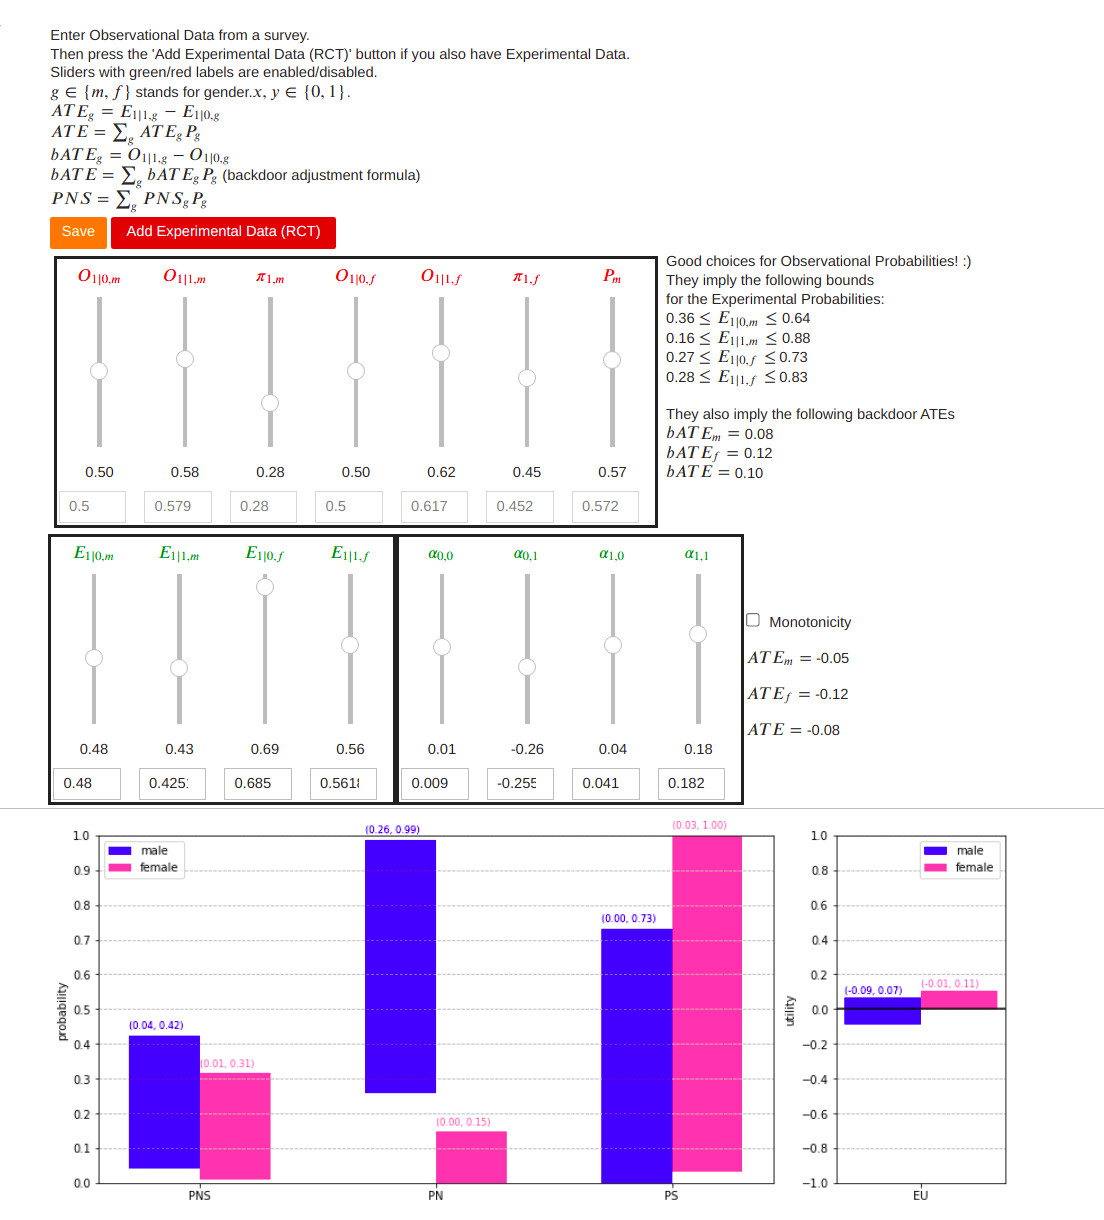
\includegraphics[width=5.5in]
{personalized/JudeasRx-screenshot.jpg}
\caption{Interface
for the Python
program JudeasRx,
with data entered
by Boris Sobolev.}
\label{fig-sobolev}
\end{figure}
